%% The following is a directive for TeXShop to indicate the main file
%%!TEX root = diss.tex

\chapter{Case Study \#2 TKC}
\label{ch:CaseStudy2}

%In all cases these are first guesses at what needs to be in each section more or less detail need to be added.



\section{Overview of Deposits}
\label{sec:Overview of Deposits:TKC}
%
%Kimberlite Complex
%Two anomalies, focusing on the southern one (DO27)
%
%Magnetic Anomaly. Remanent magnetization is likely present but largely in the direction of the earth's field
%Density Anomaly. 
\section{Discussion of the Geophysical Data Given}
\label{sec:Discussion of the Geophysical Data Given:TKC}
%
%Magnetics: Three different surveys\\
%Gravity: Ground mag (of usable but dubious quality), Gravity Gradiometry airborne data
%
%much EM as well, outside the scope of this Master's Thesis

\section{What Information is Available}
\label{sec:What Information is Available:TKC}

%Great deal of borehole data with rock units at each depth
%We also have Phys Props at various points along the holes. We can either mean these across the facies or take the value of each facies that the specially nearest the the measured result.
%
%From the borehole data we also have created a surface model of each of the units
%
%again from the borehole data, we have graphical cross section maps

\section{Synthetic Model}
\label{sec:Synthetic Model:TKC}
%
%Given the amount of \emph{a priori} information that has been collected in the region we can make a fairly non-trivial synthetic model to test various forms of constraints. The primary source of information for the creation of the synthetic model are drill hole logs of the kimberlite pipe \cite{eggleston2014peregrine}. From these drill holes, a data set representing the outer surface of the main geological units (PK and HK), was created. These are shown in \autoref{fig:TKCdataPKHK} along with the VTEM magnetic data over top of DO27, and the mesh used throughout the rest of this section.
%
%\begin{figure} [h]
%    \centering
%    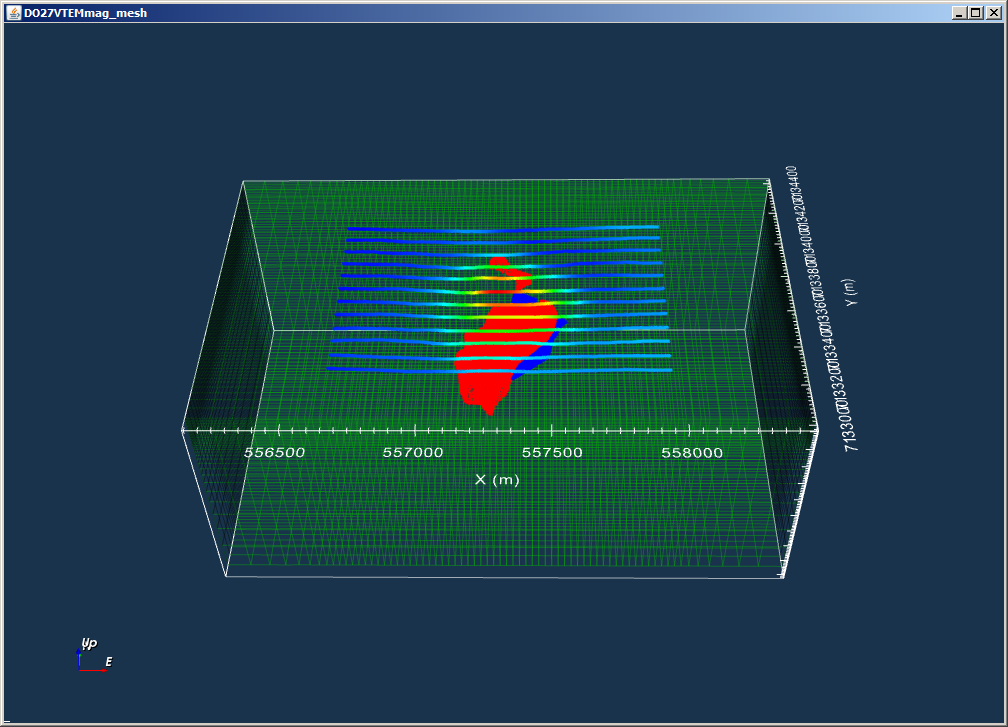
\includegraphics[width=0.8\textwidth]{images/TKC/TKCdataPKHK.PNG}
%    \caption{Mesh used in this chapter along VTEM data, and outer bound of PK (red) and HK (blue)}
%    \label{fig:TKCdataPKHK}
%\end{figure}
%
%Using the geology unit data sets and a geological model is created \autoref{fig:TKCgeoModel}. Given this geology model and using a parametric voxel inversion (this will be described in an earlier chapter) we now have a susceptibility model that closely matches know geological structure and makes an attempt at fitting the data \autoref{fig:TKCgeoModel}. For this parametric inversion result the PK unit has an effective susceptibility of .00657(SI) and the HK unit has an effective susceptibility of .0271 (SI). These numbers may seem high but it is important to note that they are effect susceptibilities and not susceptibilities. Accounting for Koenigsberger ratios of HK and PK samples from TKC the results roughly fit petrophysical measurements. The fit of this synthetic model to the true data is shown in  \autoref{fig:paramModMisfitNorm}, the effective $\Phi_d$ of the predicted data is 
%
%\begin{figure} [h]
%    \centering
%    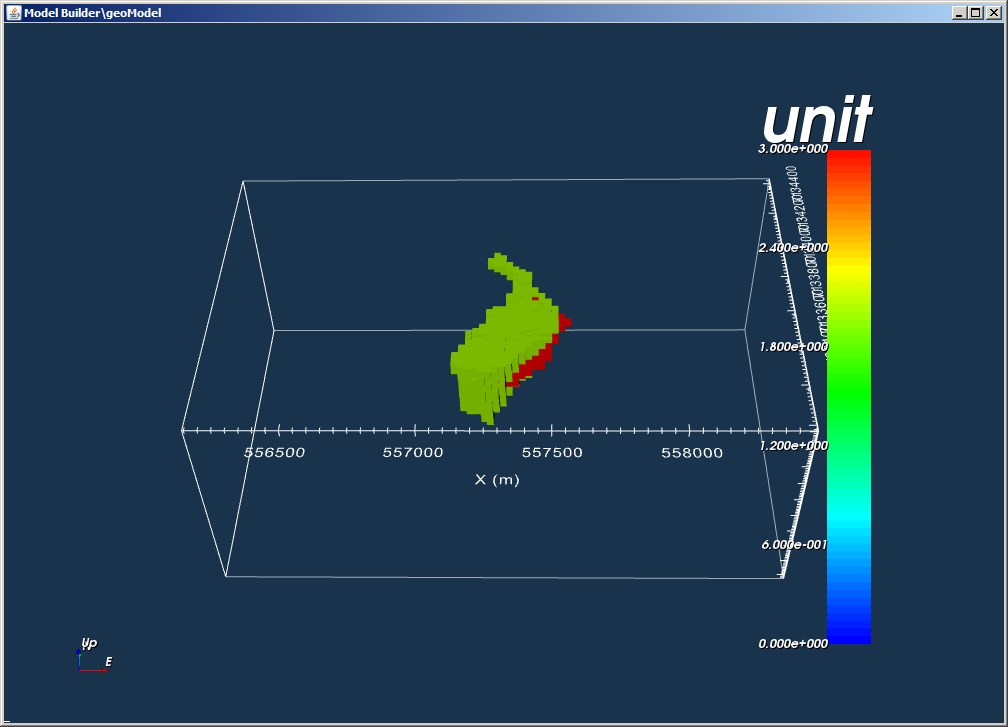
\includegraphics[width=0.8\textwidth]{images/TKC/TKCgeoModel.PNG}
%    \caption{Geology model defined by geology data sets}
%    \label{fig:TKCgeoModel}
%\end{figure}
%
%\begin{figure} [h]
%    \centering
%    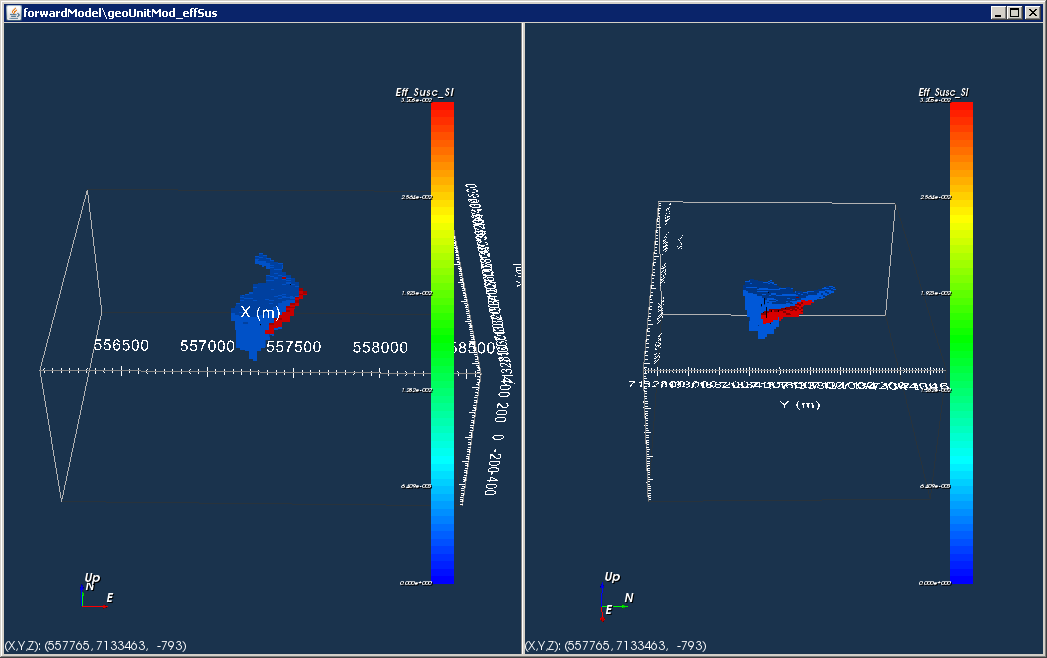
\includegraphics[width=0.8\textwidth]{images/TKC/TKCsuscModel.PNG}
%    \caption{Geology model defined by geology data sets}
%    \label{fig:TKCsuscModel}
%\end{figure}
%
%\begin{figure} [h]
%    \centering
%    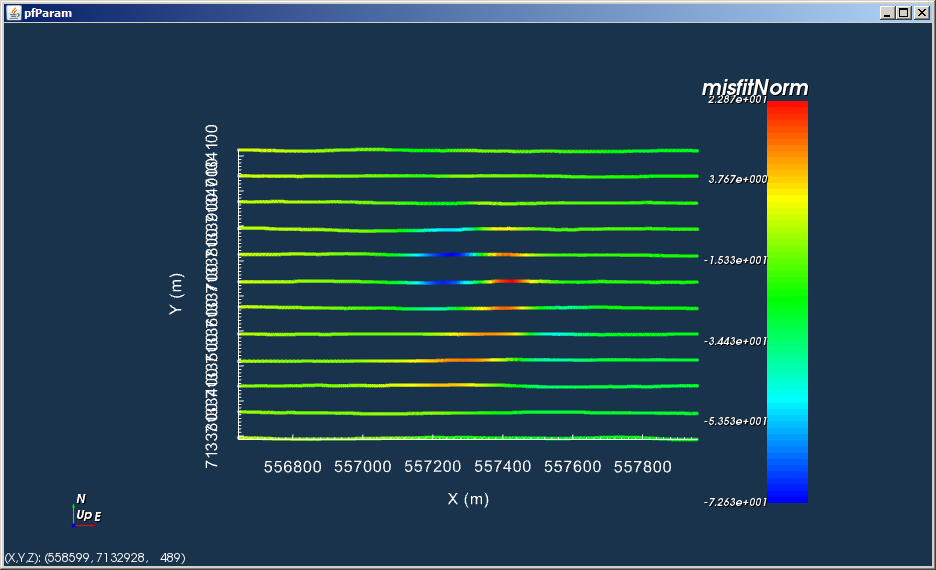
\includegraphics[width=0.8\textwidth]{images/TKC/paramModMisfitNorm.PNG}
%    \caption{Normalized misfit of parametric voxel inversion}
%    \label{fig:paramModMisfitNorm}
%\end{figure}

\FloatBarrier
\section{Blind Inversion of the Synthetic Model}
\label{sec:Blind Inversion of the Synthetic Model:TKC}

%Show results. show how model is insufficiently compact and over estimates the amount of kimberlite

\section{Determination of Magnetization Dirrection}
\label{sec:Determination of Magnetization Dirrection}
%
%Correlation of Vertical and Total Gradients of Half RTP field \cite{dannemiller2006MagDirection}
%
%taking core direction from MVI result 
%
%apply recovered direction to the anomaly direction in MAG3D
%could also use parametric inversion and MVI sensitivities to provide more constraint.
%
%could apply anomalous dirrection locally to anomaly 
%
%In any case the result will be very similar to the earth's field in the location

\section{Creation of Constraints and Types of Data}
\label{sec:Creation of Constraints:TKC}

%Extensive Boreholes with rock units
%Multiple cross sections (crreated from said bore holes)
%Multiple data types to cluster



\subsection{$\alpha$ coefficients}
\label{sec:alpha coefficients:TKC}

%not much with alphas to be done here given that we don't expect discontinuity in any one particular dirrection.

\subsection{Reference Models}
%\label{sec:Reference Models:TKC}
%
%Most work to be done here. 
%
%We can create a reference model from the phys prop results from the borehole data. Perhaps we should only use some of the boreholes so that we have a more realistic amount of information than in a fully drilled example. We have two ways of applying phys prop measures to inversion and might use both. Also using $K_n$s to improve degree of fit between phys prop measures and effective susc recovered properties
%(show reference model)
%(show result)
%
%with sufficient boreholes we could make a incorrect surface that approximates the ``true'' model used. Use this with parametric inversion for reference model
%(show reference model)
%(show result)
%
%using clustering between density and mag (and conductivity and chargeablity) to create clusters, populate each cluster with a value either the mean value of the cluster or a parametric inversion and use as reference
%(show reference model)
%(show result)
%
%use cross section from \cite{harder2006geologyTKC}
%perhaps extend away from line and down weight
%(show reference model)
%(show result)
%
%(show Combined result)

\subsection{Weighting matrices}
\label{sec:Weighting matrices:TKC}
%
%smallness: using some measure of confidence in the measures decrease in cells with reference model specified to force the result to approximate the reference model. In case the cross section is extended down I will lower the $W_s$ as model cells are further away from the cross section
%(show smallness weight model)
%(show result, compare to result without)
%
%smoothness: to spread the model values away from where they are specified I can increase the smoothness weights in the vicinity of cells with specified reference models. 
%(show face weight model)
%
%with sufficient boreholes we could make a incorrect surface that approximates the ``true'' model used. Use this with parametric inversion for reference mode,l put lower weights along this surface.
%(show face weight model)
%
%using clustering between density and mag (and conductivity and chargeablity) to create clusters, populate each cluster with a value either the mean value of the cluster or a parametric inversion and use as reference
%(show result)
%
%(show result, compare to result without)
%
%(show Combined result)
\subsection{Bounds}
\label{sec:Bounds:TKC}
%
%Also useful for forcing model values to be near the specified reference model while allowing for uncertainty in our phys prop value. Since we have more statistical info on the 
%(show result)
%
%Need to determine if showing the field example is worthwhile at this point and how to bring it into the narrative

\endinput

Any text after an \endinput is ignored.
You could put scraps here or things in progress.
